% ===========================
%       Chapter 1A.2
%       Motion Graphs
%   Created by Michael Tang
%        2025.01.18
% ===========================

\subsubsection{1A.2 Motion Graphs}
\paragraph{Displacement-Time Graphs}
\begin{itemize}
    \item \textbf{Definition:} Tracks the position of an object over time.
    \item \textbf{Key Features:}
    \begin{itemize}
        \item \textbf{Gradient:} Represents the velocity of the object.
        \begin{equation}
            v = \frac{\Delta s}{\Delta t}
        \end{equation}
        \item \textbf{Straight Line:} Constant velocity.
        \item \textbf{Curved Line:} Changing velocity (acceleration or deceleration).
        \item \textbf{Flat Line:} Object is stationary.
    \end{itemize}
    \begin{figure}[H]
        \centering
        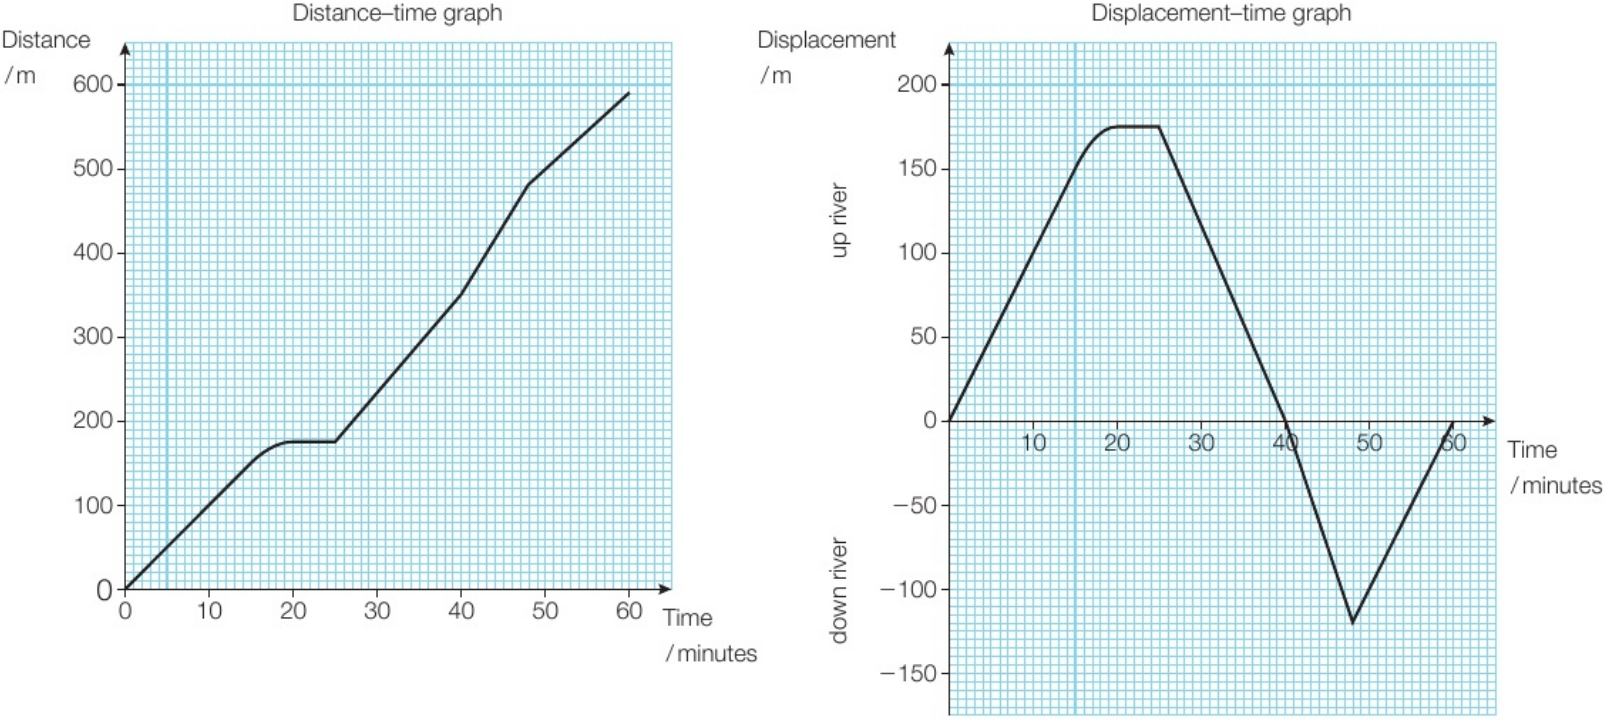
\includegraphics[scale=0.15]{Physics/1A/Images/1A-2-1.png}
    \end{figure}
    \item \textbf{Example:} According to the graph above, from 0-15 minutes, boat travels 150 m up to the river.
    \begin{equation}
        v = \frac{\Delta s}{\Delta t} = \frac{150}{\left(15 - 0\right) \times 60} = 0.167 \text{m/s}
    \end{equation}
\end{itemize}

\paragraph{Velocity-Time Graphs}
\begin{itemize}
    \item \textbf{Definition:} Shows velocity of an object over time.
    \item \textbf{Key Features:}
    \begin{itemize}
        \item \textbf{Gradient:} Represents the acceleration of the object.
        \begin{equation}
            a = \frac{\Delta v}{\Delta t}
        \end{equation}
        \item \textbf{Area Under Graph:} Total distance traveled by the object.
        \begin{equation}
            d = v \times t
        \end{equation}
        \item \textbf{Positive / Negative Gradient:} Direction of velocity (up / down motion).
    \end{itemize}
    \begin{figure}[H]
        \centering
        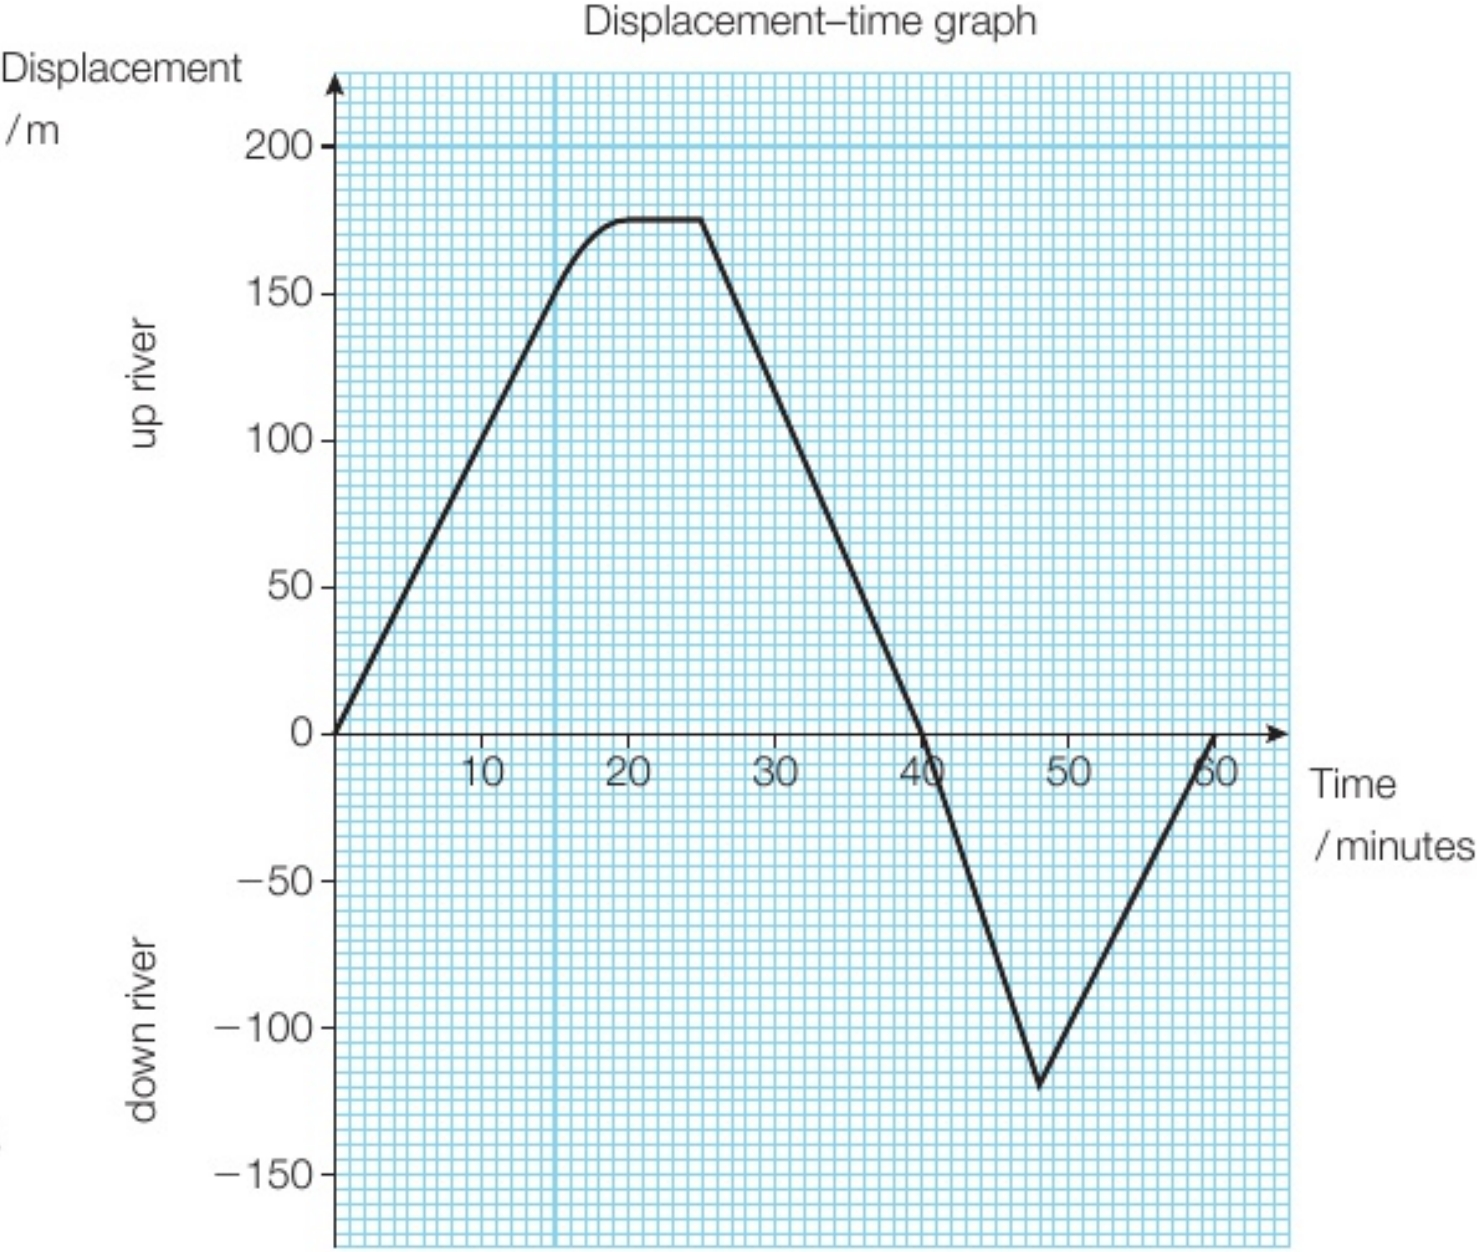
\includegraphics[scale=0.15]{Physics/1A/Images/1A-2-2.png}
    \end{figure}
    \item \textbf{Example:} According to the graph above, acceleration is zero (flat line at $0.167$ m/s). Calculate the
    acceleration between 15-20 minutes.
    \begin{equation}
        a = \frac{v - u}{t} = \frac{0 - 0.167}{\left(20 - 15\right) \times 60} = -0.0006 \text{m/s}^2
    \end{equation}
\end{itemize}

\paragraph{Acceleration-Time Graphs}
\begin{itemize}
    \item \textbf{Definition:} Represents acceleration over time.
    \item \textbf{Key Features:}
    \begin{itemize}
        \item \textbf{Flat Line Above Zero:} Constant positive acceleration.
        \item \textbf{Flat Line Below Zero:} Constant negative acceleration (deceleration).
        \item \textbf{Area Under Graph:} Change in velocity.
    \end{itemize}
    \begin{figure}[H]
        \centering
        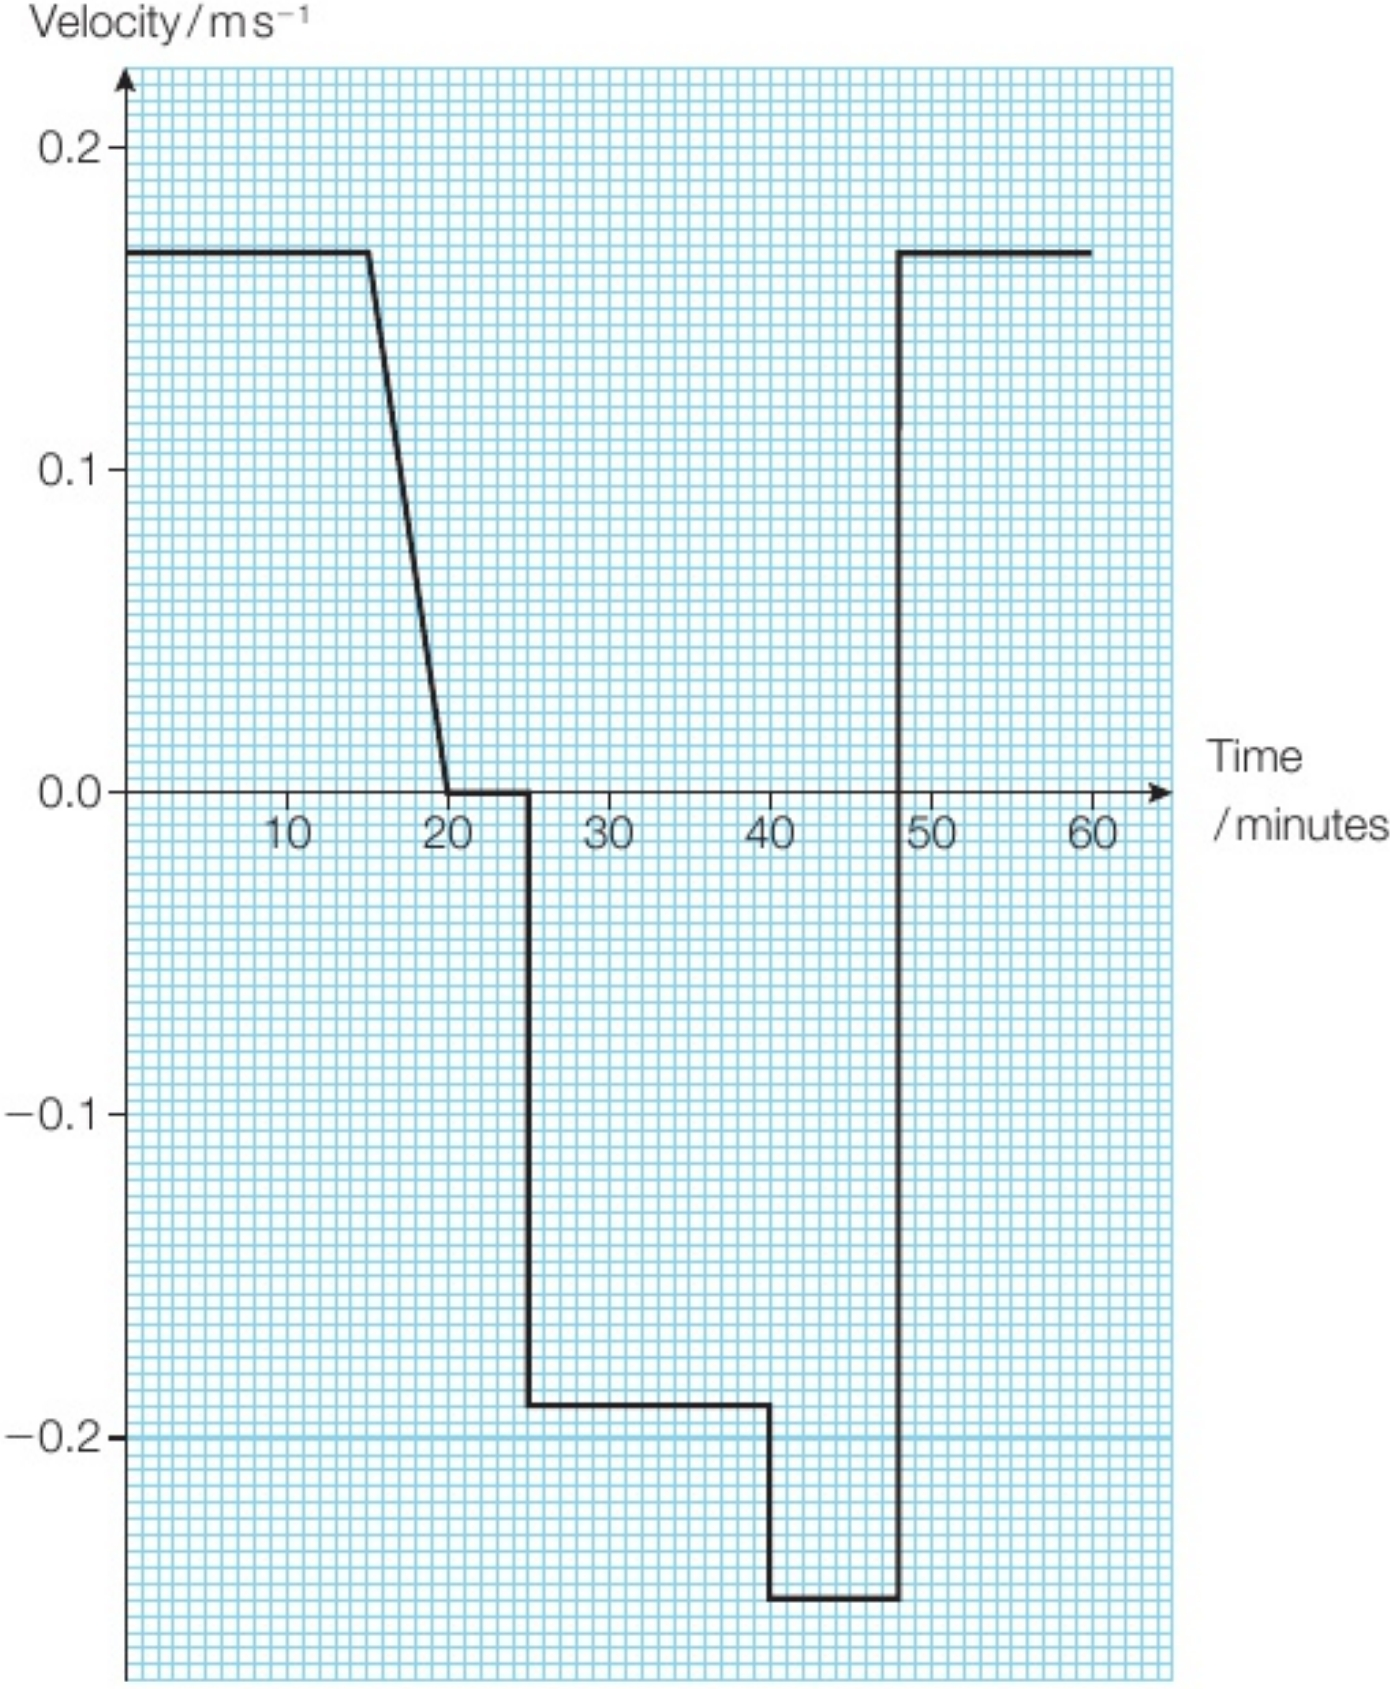
\includegraphics[scale=0.15]{Physics/1A/Images/1A-2-3.png}
    \end{figure}
\end{itemize}

\paragraph{Multiflash Photography}
\begin{itemize}
    \item \textbf{Method:} Use time intervals and measure distance to calculate acceleration due to gravity.
    \item \textbf{Observations:} Observations are plotted to create accurate velocity-time graphs.
\end{itemize}